%%%%%%%%%%%%%%%%%%%%%%%%%%%%%%%%%%%%%%%%%%%%%%%%%%%%%%%%%%%%%%%%%%%%%%%%%%%%%%%%
\chapter{Proof of Concepts and Validation}\label{ch:validation}
%%%%%%%%%%%%%%%%%%%%%%%%%%%%%%%%%%%%%%%%%%%%%%%%%%%%%%%%%%%%%%%%%%%%%%%%%%%%%%%%


%%%%%%%%%%%%%%%%%%%%%%%%%%%%%%%%%%%%%%%%%%%%%%%%%%%%%%%%%%%%%%%%%%%%%%%%%%%%%%%%'
\section{Validation Tests}


As proof of concepts for our tool, we are going to use Mininet's emulated testbeds. We automate all tests using scripts, so our experiments are fully reproducible. They are responsible for running all the proposed tests in this chapter and perform the calculations. It includes:

\begin{itemize}
    \item Build the topology;
    \item Run the SIMITAR traffic generator;
    \item Collect the packeckets as \textit{pcap} files, and stract data from it;
    \item Perform the proposed proof of concept analysis;
    \item Plot the data.
\end{itemize}

Each test is organized as a Python package, responsible for trigger all the applications and procedures. A \textit{config.py} file can configure the parameters for each simulation. The files \textit{README} on each package, provide a tutorial to run each test correctly. With all tools installed, less then fifteen minutes is enough for rerunning each test. A complete specification of our scenario we show at the table ~\ref{tab:specifications}, including the hardware specifications and the software versions. 

\begin{table}[ht!]
    \centering
    \caption{Experiments specification table}
    \label{tab:specifications}
    \begin{tabular}{ll}
        \hline
        Processor            & Intel(R) Core(TM) i7-4770, 8 cores, CPU @ 3.40GHz \\
        RAM                  & 15.5 GB                                           \\
        HD                   & 1000 GB                                           \\
        Linux         & 4.8.0-59-generic                                  \\
        Ubuntu        & Ubuntu 16.10 (yakkety)                            \\
        SIMITAR       & v0.4.2 (Eulemur rubriventer)                      \\
        Mininet       & 2.3.0d1                                           \\
        Iperf         & iperf version 2.0.9 (1 June 2016) pthreads        \\
        Libtins       & 3.4-2                                             \\
        OpenDayLight  & 0.4.0-Beryllium                                   \\
        Octave        & 4.0.3                                             \\
        Pyshark       & 0.3.6.2                                     \\
        Wireshark     & 2.2.6+g32dac6a-2ubuntu0.16.10               \\
        Tcudump       & 4.9.0 \\
        libpcap       & 1.7.4\\
        \hline
    \end{tabular}
\end{table}

\begin{figure}[!ht]
    \centering
    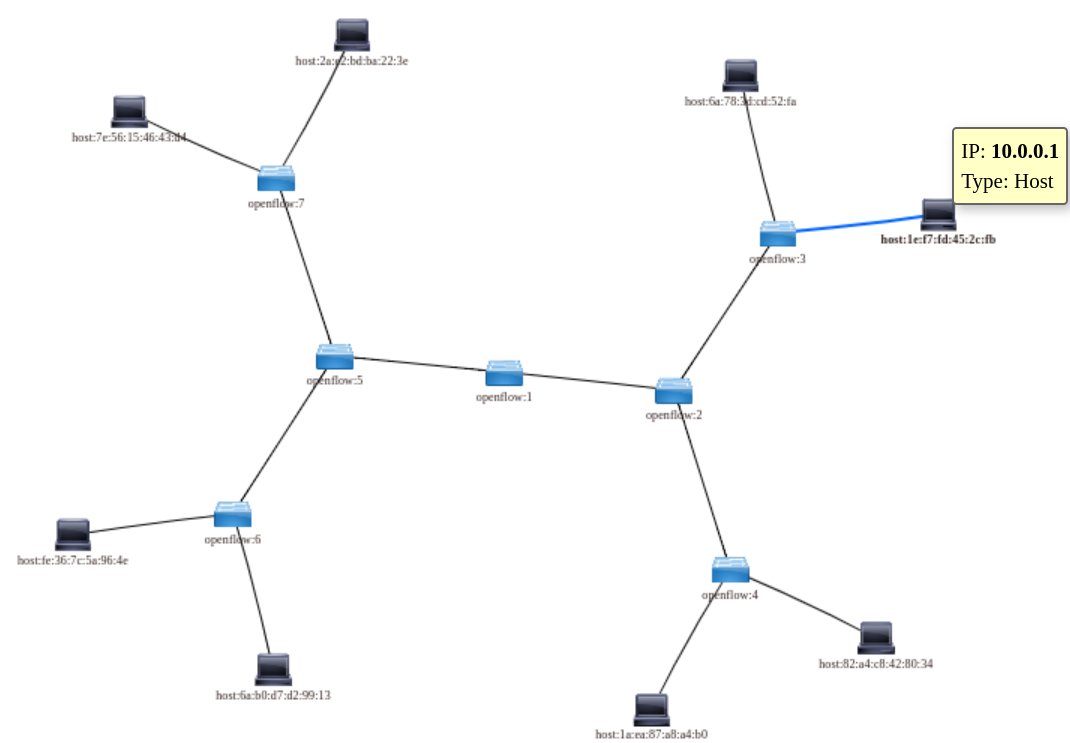
\includegraphics[scale=0.4]{figures/ch5/topo-tree}
    \caption{Tree SDN topology emulated by mininet, and controlled by OpenDayLight Beryllium}
    \label{fig:topo-tree}
\end{figure}

\begin{figure}[!ht]
    \centering
    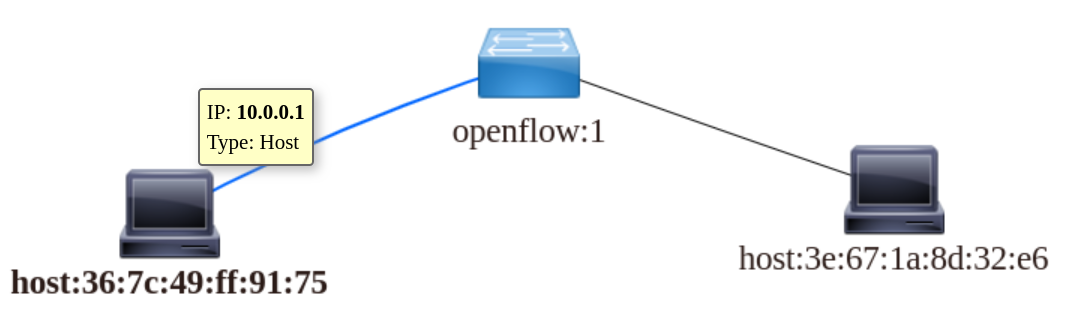
\includegraphics[scale=0.4]{figures/ch5/topo-simple}
    \caption{Single hop SDN topology emulated by mininet, and controlled by OpenDayLight Beryllium}
    \label{fig:topo-simple}
\end{figure}


For each test, we generate a set of plots to compare the original and synthetic trace. Two of them we use for visual comparison: flows per second and bandwidth. To examine the realism quality of the generated traffic, we plot the flows cumulative distribution function (CDF)\cite{harpoon-paper}, and the Wavelet multiresolution analysis.  In every case, the closer the plots are, the more similar are the traces. Also, we wrote on the table ~\ref{tab:results-summary} a compilation of each traffic statistics. 

The flow's cumulative distribution measures each new flow identified the trace. It is a measure similarity of the traffic at the flow-level.  The wavelet multiresolution analysis is capable of capture traffic scaling characteristics and is a measure of similarity at the packet-level. If the value decreases, a periodicity on that time scale exists. With white-noise features, the traffic will remain constant. If the traffic has self-similar characteristics on a particular time scale, its value will increase linearly. We show a sumary of all performed tests on table~\ref{tab:validation-tests-performed}.


\begin{table}
	\centering
	\label{tab:validation-tests-performed}
	\caption{Performed validations}
		\begin{tabular}{c c}
			\toprule
			\textbf{Metric Type} & \textbf{Validations} \\
			\midrule
			\makecell{Packet Based \\Metrics}                & \makecell{Data bit rate (kbps), Average packet\\
				rate (packets/s), Average packet size\\
				(bytes), Number of packets, Number of\\
				packets, Bandwidth over time}\\
			
			\makecell{Flow Based \\ Metrics}                & \makecell{Number of flows, Flows per second, \\
				Flows CDF distributions}\\
			
			\makecell{Fractal and Scaling \\ Characteristics} & \makecell{Hurst Exponent, Wavelet \\
				Multiresolution Analisis}\\
			\bottomrule
		\end{tabular}

\end{table}


We use as testbeds: a tree topology (figure~\ref{fig:topo-tree}), similar to tests performed by Swing\cite{swing-paper}\cite{background-traffic-matter}\cite{legotg-paper}, and a one-hop connection of two hosts. Both topologies are SDN networks and have OpenDayLight Beryllium as the controller.

For generating the traffic on the host \textit{h1} with IPv4 address 10.0.0.1. The traffic is captured from the host interface with TCPdump in a \textit{pcap} format.  We organized the project directory tree as follows\footnote{ \href{https://github.com/AndersonPaschoalon/ProjetoMestrado}{https://github.com/AndersonPaschoalon/ProjetoMestrado} }: the software is at \textit{SIMITAR}. All validation tests and project prototypes we aved at \textit{Tests} directory. The software documentation is at \textit{Docs} directory.

We use SIMITAR v0.4.2 (Eulemur rubriventer)\footnote{ We label the tags of SIMITAR control version on GitHub as lemurs species names (\href{https://en.wikipedia.org/wiki/List_of_lemur_species}{https://en.wikipedia.org/wiki/List\_of\_lemur\_species})}, as tagged at the GitHub repository.  SIMITAR already have two functional traffic generator engines: Iperf and libtins C++ API.  

For schedule of the timing of traffic generated by each flow, we implemented three methodologies: \texttt{usleep()} C function,\texttt{select()} C function and \textit{pooling}. Here we use \texttt{usleep()} . We implemented the class \texttt{IperfFlow,} responsible for generate the traffic of each flow, using \texttt{popen()} and \texttt{pclose()} to instantiate Iperf processes, responsible for generating the traffic. Traffic customization on Iperf has many limitations. It cannot assign arbitrary IP addresses as source and destination since it must establish a connection between the source and destination. For the transport layer, it supports TCP and UDP protocol, and constant bandwidth traffic. On the other hand, it enables customization of transmission time, number of packets, windows size, TTL, packet sizes, payload and many other features. Since Iperf has to establish a communication, SIMITAR must operate in the client mode on the source, and server mode on the destinations.

Libtins enable the creation and emission of arbitrary packets and do not require the establishment of a connection.  Thus SIMITAR does not need to operate in server mode on the destination. The packet customization capability is vast, and enable a full usage of our model parameters. Control inter-packet times stays for future work~\ref{ch:conclusion}. 





%%%%%%%%%%%%%%%%%%%%%%%%%%%%%%%%%%%%%%%%%%%%%%%%%%%%%%%%%%%%%%%%%%%%%%%%%%%%%%%%
\section{Results}


\begin{table}[ht!]
    \centering
    \caption{Sumary of results comparing the original traces (italic) and te traffic generated by SIMITAR, with the description of the scenario.}
    \label{tab:results-summary}
    \scalebox{0.87}{
\begin{tabular}{lcccccc}
    \hline
    \multicolumn{1}{c}{\multirow{3}{*}{}} & \multirow{3}{*}{\textit{skype-pcap}} & \multicolumn{1}{c}{\multirow{3}{*}{\begin{tabular}[c]{@{}c@{}}skype, \\ one-hop, \\ iperf\end{tabular}}} & \multicolumn{1}{c}{\multirow{3}{*}{\begin{tabular}[c]{@{}c@{}}skype, \\ tree, \\ iperf\end{tabular}}} & \multicolumn{1}{c}{\multirow{3}{*}{\begin{tabular}[c]{@{}c@{}}skype, \\ one-hop, \\ libtins\end{tabular}}} & \multirow{3}{*}{\textit{lgw10s-pcap}} & \multicolumn{1}{c}{\multirow{3}{*}{\begin{tabular}[c]{@{}c@{}}lgw10s, \\ one-hop, \\ libtins\end{tabular}}} \\
    \multicolumn{1}{c}{}                  &                             & \multicolumn{1}{c}{}                                                                                     & \multicolumn{1}{c}{}                                                                                  & \multicolumn{1}{c}{}                                                                                       &                              & \multicolumn{1}{c}{}                                                                                        \\
    \multicolumn{1}{c}{}                  &                             & \multicolumn{1}{c}{}                                                                                     & \multicolumn{1}{c}{}                                                                                  & \multicolumn{1}{c}{}                                                                                       &                              & \multicolumn{1}{c}{}                                                                                        \\ \hline
    Hurst Exponent                        & 0.601                       & 0.618                                                                                                    & 0.598                                                                                                 & 0.691                                                                                                      & 0.723                        & 0.738                                                                                                       \\
    Data bit rate (kbps)                  & 7                           & 19                                                                                                       & 19                                                                                                    & 12                                                                                                         & 7252                         & 6790                                                                                                        \\
    Average packet rate (packets/s)       & 3                           & 4                                                                                                        & 5                                                                                                     & 6                                                                                                          & 2483                         & 2440                                                                                                        \\
    Average packet size (bytes)           & 260,89                      & 549,05                                                                                                   & 481,14                                                                                                & 224,68                                                                                                     & 365,00                       & 347,85                                                                                                      \\
    Number of packets                     & 1071                        & 1428                                                                                                     & 1604                                                                                                  & 2127                                                                                                       & 24 k                         & 24 k                                                                                                        \\
    Number of flows                       & 167                         & 350                                                                                                      & 325                                                                                                   & 162                                                                                                        & 3350                         & 3264                                                                                                        \\ \hline
\end{tabular}
    }
\end{table}



% Bandwidth
\begin{figure}[h!]
    \centering
    \subfloat[\textit{Iperf, single-hop, skype-pcap}]{
        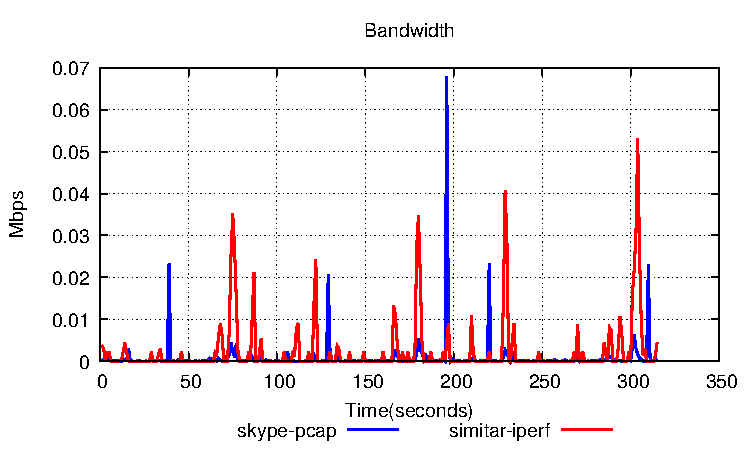
\includegraphics[width=77mm]{figures/ch5/skype-iperf-Bandwidth.pdf}
        \label{fig:iperfBw}
    }
    \hspace{0mm}
    \subfloat[\textit{Iperf, tree, skype-pcap}]{
        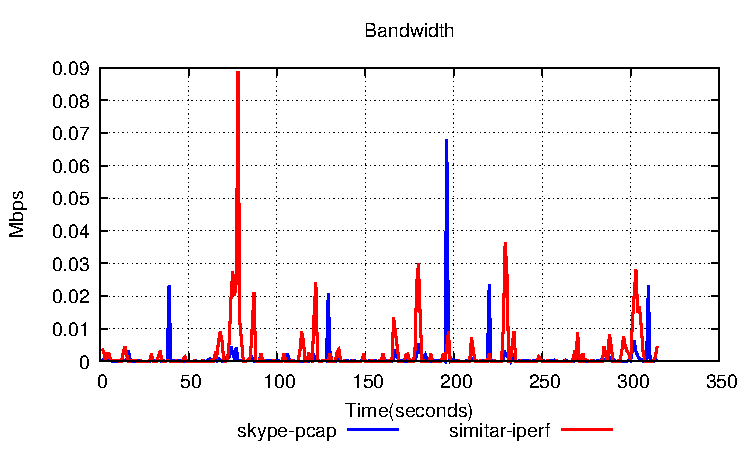
\includegraphics[width=77mm]{figures/ch5/skype-tree-iperf-Bandwidth.pdf}
        \label{fig:iperftreeBw}
    }
    \hspace{0mm}
    \subfloat[\textit{libtins, single-hop, skype-pcap}]{
        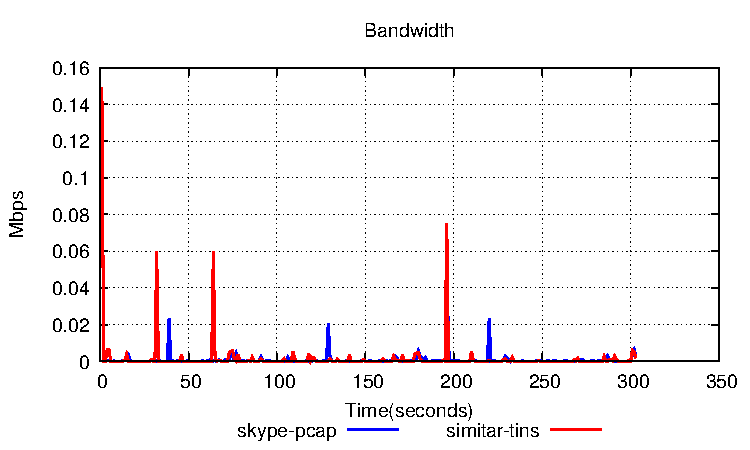
\includegraphics[width=77mm]{figures/ch5/skype-tins-Bandwidth.pdf}
        \label{fig:tinsBw}
    }
    \hspace{0mm}
    \subfloat[\textit{libtins, single-hop, langw10s-pcap}]{
        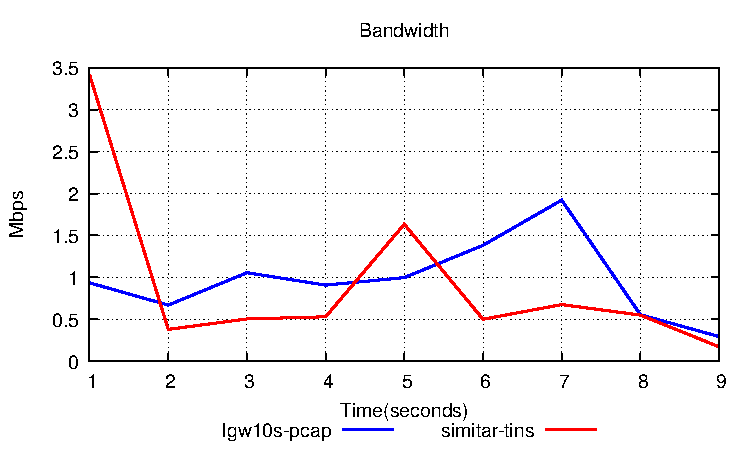
\includegraphics[width=77mm]{figures/ch5/lgw-tins-Bandwidth.pdf}
        \label{fig:tinsLgwBw}
    }
    \hspace{0mm}
    \caption{Traces bandwidth.}
    \label{fig:flows-bandwidth}
\end{figure}
% Flows per second
\begin{figure}[ht!]
    \centering
    \subfloat[\textit{Iperf, single-hop, skype-pcap}]{
        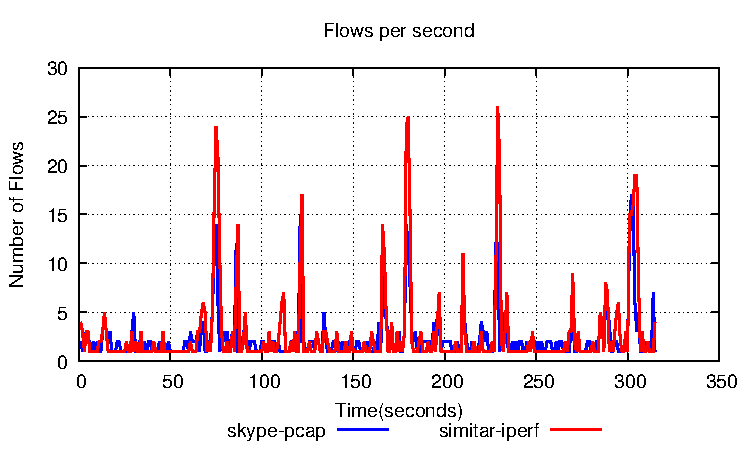
\includegraphics[width=77mm]{figures/ch5/skype-iperf-FlowsPs.pdf}
        \label{fig:iperfFps}
    }
    \hspace{0mm}
    \subfloat[\textit{Iperf, tree, skype-pcap}]{
        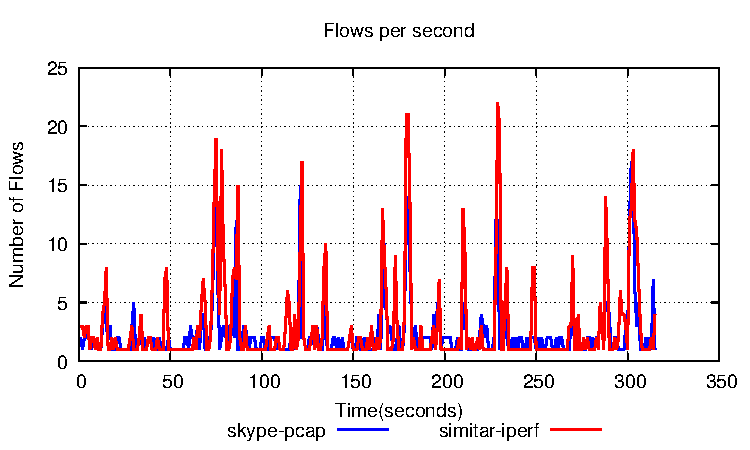
\includegraphics[width=77mm]{figures/ch5/skype-tree-iperf-FlowsPs.pdf}
        \label{fig:iperftreeFps}
    }
    \hspace{0mm}
    \subfloat[\textit{libtins, single-hop, skype-pcap}]{
        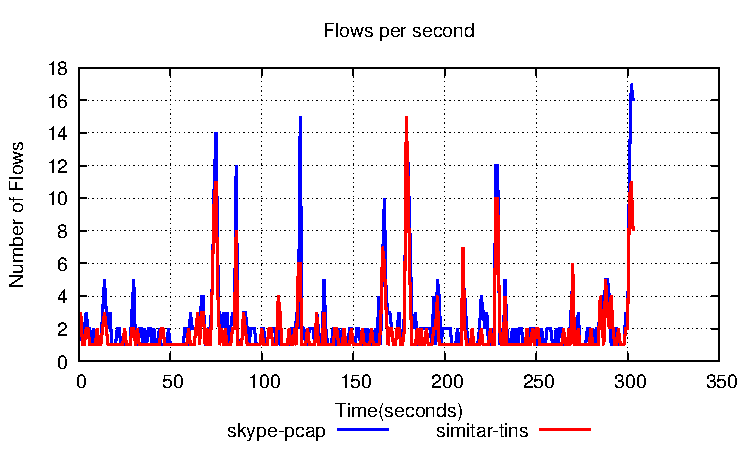
\includegraphics[width=77mm]{figures/ch5/skype-tins-FlowsPs.pdf}
        \label{fig:tinsCdf}
    }
    \hspace{0mm}
    \subfloat[\textit{libtins, single-hop, langw10s-pcap}]{
        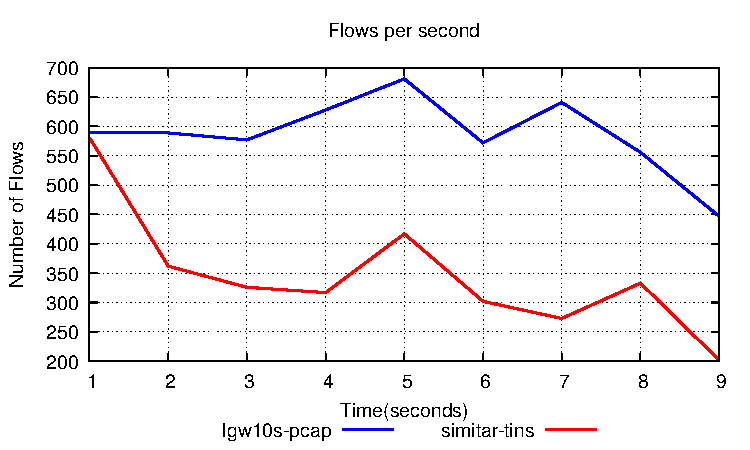
\includegraphics[width=77mm]{figures/ch5/lgw-tins-FlowsPs.pdf}
        \label{fig:tinsLgwFps}
    }
    \hspace{0mm}
    \caption{Flow per seconds}
    \label{fig:flows-ps}
\end{figure}
% Flow CDF
\begin{figure}[ht!]
    \centering
    \subfloat[\textit{Iperf, single-hop, skype-pcap}]{
        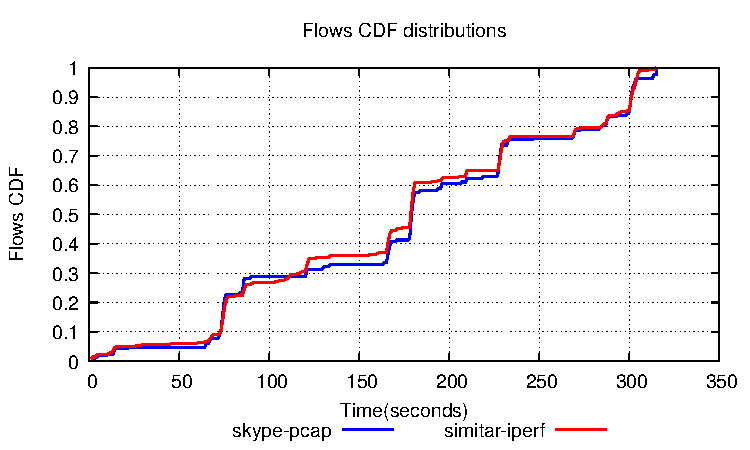
\includegraphics[width=77mm]{figures/ch5/skype-iperf-FlowCdf.pdf}
        \label{fig:iperfCdf}
    }
    \hspace{0mm}
    \subfloat[\textit{Iperf, tree, skype-pcap}]{
        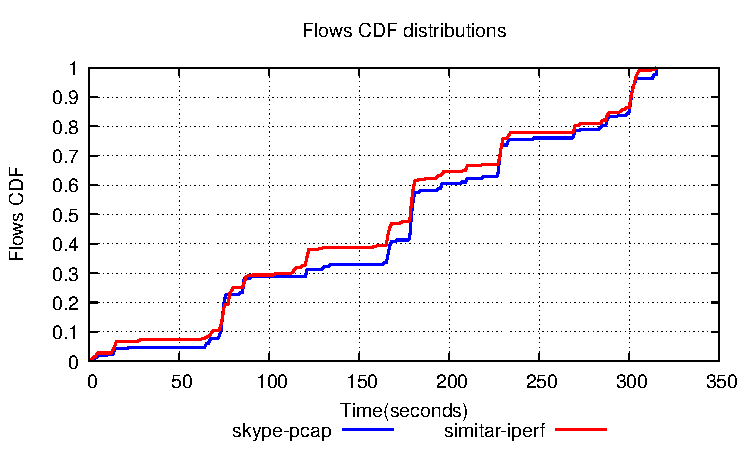
\includegraphics[width=77mm]{figures/ch5/skype-tree-iperf-FlowCdf.pdf}
        \label{fig:iperftreeCdf}
    }
    \hspace{0mm}
    \subfloat[\textit{libtins, single-hop, skype-pcap}]{
        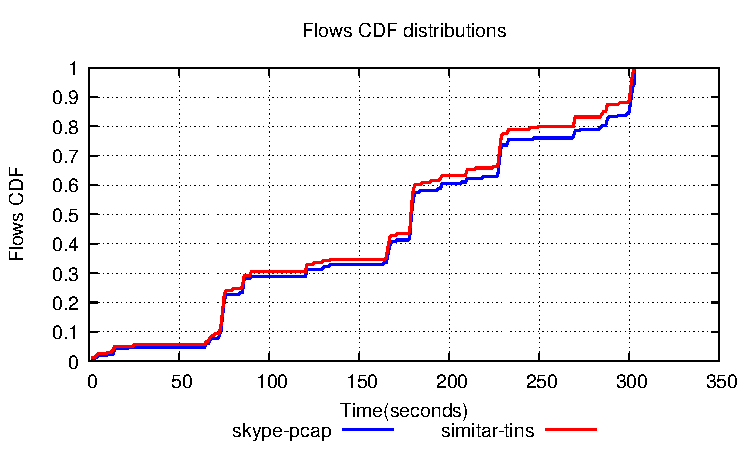
\includegraphics[width=77mm]{figures/ch5/skype-tins-FlowCdf.pdf}
        \label{fig:tinsCdf}
    }
    \hspace{0mm}
    \subfloat[\textit{libtins, single-hop, langw10s-pcap}]{
        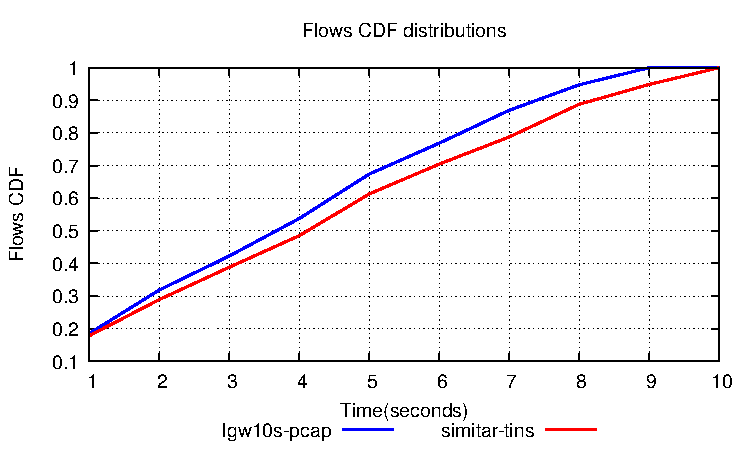
\includegraphics[width=77mm]{figures/ch5/lgw-tins-FlowCdf.pdf}
        \label{fig:tinsLgwCdf}
    }
    \hspace{0mm}
    \caption{Flows cumulative distributions.}
    \label{fig:flows-cdf}
\end{figure}
% Wabelet
\begin{figure}[h!]
    \centering
    \subfloat[\textit{Iperf, single-hop, skype-pcap}]{
        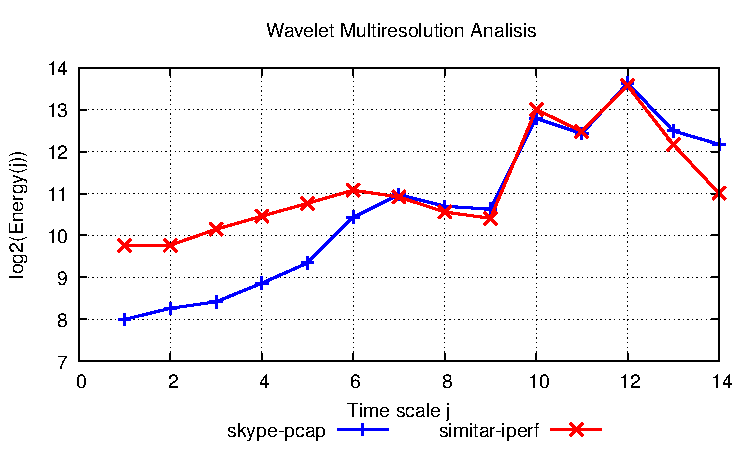
\includegraphics[width=77mm]{figures/ch5/skype-iperf-WaveletMREA.pdf}
        \label{fig:iperfWaveletMREA}
    }
    \hspace{0mm}
    \subfloat[\textit{Iperf, tree, skype-pcap}]{
        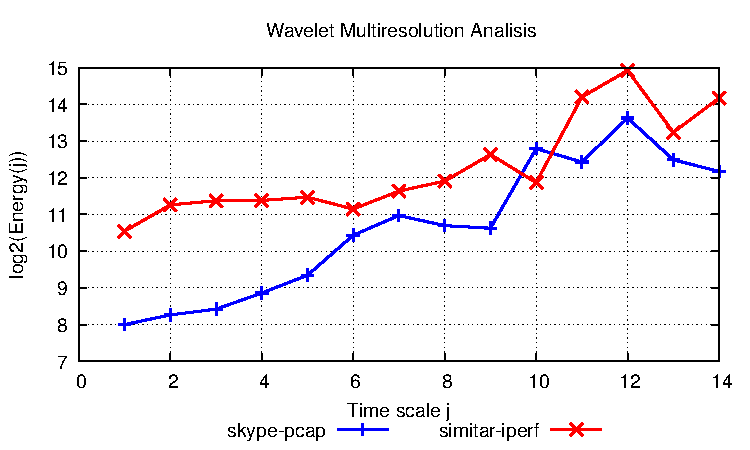
\includegraphics[width=77mm]{figures/ch5/skype-tree-iperf-WaveletMREA.pdf}
        \label{fig:iperftreeWaveletMREA}
    }
    \hspace{0mm}
    \subfloat[\textit{libtins, single-hop, skype-pcap}]{
        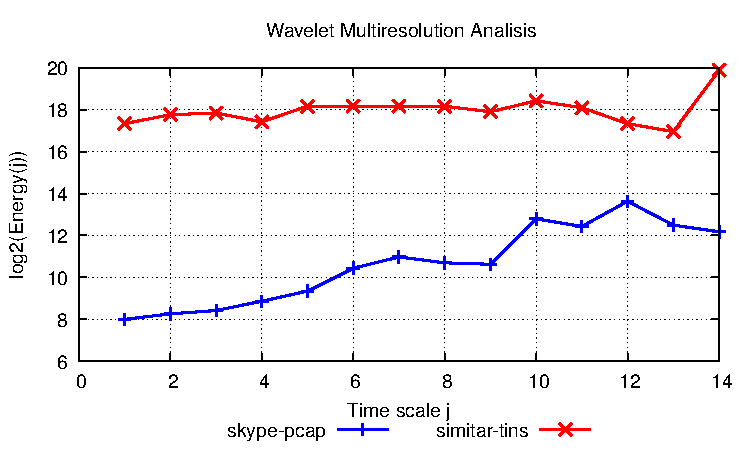
\includegraphics[width=77mm]{figures/ch5/skype-tins-WaveletMREA.pdf}
        \label{fig:tinsWaveletMREA}
    }
    \hspace{0mm}
        \subfloat[\textit{libtins, single-hop, langw10s-pcap}]{
            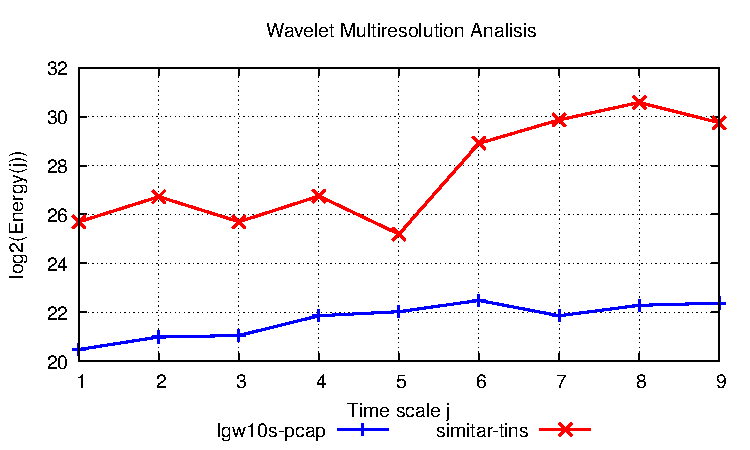
\includegraphics[width=77mm]{figures/ch5/lgw-tins-WaveletMREA.pdf}
            \label{fig:tinsLgwWaveletMREA}
        }
        \hspace{0mm}
    \caption{Wavelet multiresolution energy analysis.}
    \label{fig:wavelet}
\end{figure}


We display our results in the figures ~\ref{fig:flows-ps} to ~\ref{fig:wavelet}, and in the table ~\ref{tab:results-summary}, where the original and the synthetic traffics are compared. As we can see in the figure ~\ref{fig:flows-bandwidth}, the generated traffics are not identical regarding bandwidth, however both presents fractal-like shape. The Hurst exponent of inter-packet times in every case has an error smaller than 10\% compared to the original in every case. This result indicates that in fact, the fractal-level of each synthetic traffic is indeed similar to the original.  

The plot of flows per second seems much more accurate visually since most of the peaks match.  Indeed, no visual lag between the plots. We can analyze it precisely observing the cumulative flow distribution\ref{fig:flows-cdf}, where the results were almost identical on every plot. However, when SIMITAR is replicating the traffic of \textit{lgw10s-pcap} the number of flows per second decreases. It happens because of the methodology of traffic generation of the class \textit{TinsFlow} since it sends the packets of each stream as fast as possible. So each flow occurrence is restricted to smaller intervals. This behavior can be observed as well in the bandwidth plot. It is much more significant in the first seconds and small in  the end.

The best results achieved by SIMITAR were on the flow distribution characterization. On every experiment made, the cumulative distribution of flows was almost identical. The small imprecisions on the plots are expected and should result from threads and process concurrence of resources and imprecision on the sleep/wake signaling on the traffic generation side. Imprecisions on packet capture buffer may count as well since the operating system did the packet timing. This was our most significant achievement in our research. This result means that our method of flow scheduling and independent traffic generation were effective and efficient on replicating the original traffic at the flow-level. The actual number of flows was much more significant when SIMITAR used Iperf and about the same amount but little small when used libtins. This discrepancy happens with Iperf because it establishes additional connections to control the signaling and traffic statistics.  So, this more substantial number of flows comes from accounting, not just the traffic connections, but also with the signaling as well.  With libtins, the number of flows is small, because, if it fails to create a new traffic flow, this flows generation execution is aborted. 

On Wavelet multiresolution analysis of inter-packet times, the results have changed more in each case. The time resolution chosen was ten milliseconds, and it is represented in $\log_2$ scale. The actual time pf each time-scale $j$ value is given by the equation:

\begin{equation}
t = \frac{2^{j}}{100} [s]
\end{equation}

In the first case (figure ~\ref{fig:iperfWaveletMREA}), SIMITAR using Iperf in a single-hop scenario, on small time scales the energy level of the synthetic traffic remained almost constant, which indicates white-noise characteristics. The original skype traffic increased linearly, an indication of fractal shape. The synthetic trace started to grow at the time scale 5-6 (300-600 milliseconds). After this scale, the error between the curves become very small. One possible reason for this behavior is the fact that the constant which regulate the minimum burst time (\texttt{DataProcessor::m\_min\_on\_time}) is set to 100 milliseconds. For small time scales the traffic become similar to white noise since Iperf emits traffic with constant bandwidth. For larger time-scales, it captures the same fractals patterns of the original trace. It also captures a periodicity pattern at the time-scale of 9 seconds. The authors of \cite{swing-paper} measured the same periodicity pattern. But on this trace, we observe some periodicity at 11 and 13 time-scales (20 and 80 seconds). 

In the second case, on a tree topology on small time scales, the same white-noise behavior is identified. We identify a similar response for energy on larger time-scales, but with a more significant gap between the curves. Packet collision on switches requiring retransmission packets explains this behavior. In fact, as we can see in the table ~\ref{tab:results-summary}, two hundred more packets are leaving the client on the tree topology compared to the one-hop. 

On the last two plots, where we use libtins as packet crafter, the energy level is much higher, and the curves are much less correlated. SIMITAR are not modeling inter-packet with libtins, and are sending packets as fast as possible. We may observe on the figures ~\ref{fig:tinsBw} and ~\ref{fig:tinsLgwBw} that than have much  higher peaks compared to the original \textit{skype-pcap}.  As we see in the figure ~\ref{fig:tinsBw}, it just captured some periodicity characteristics at the time larger than 11-12 (20-40 seconds). SIMITAR determines larger periods between packets with session OFF times, and the session cut time (\texttt{DataProcessor::m\_session\_cut\_time}) is 30 seconds, that explain this behavior.


The current implementation still has problems on accurately reproduce \textit{pcaps} with high bandwidth values and a more substantial number of flows. The primary limitation is the time required to generate the trace descriptor.  The procedure is still mono-thread, and the linear regression procedure is not optimized. Although creating a trace descriptor of a small pcap file is fast, the time for processing large pcap file with thousands of flows is still prohibitively high, spending dozens of hours. 

Using the first 10 seconds of the trace \textit{bigFlows-pcap}, on 10 seconds of operation, Iperf generated much fewer packets than the expected. It is supposed behavior since the operating system couldn't handle so much newer processes (one per flow) in such short time. On the other hand, the same drawback wasn't observed using libtins as traffic generator tool, since being a low-level API makes it much computationally cheaper.  Some others unexpected behavior must have a more in-depth investigation, such as libtins generating more packets than expected for \textit{skype-pcap}, but not for \textit{lgw10s-pcap}, and why the creation of some flows fail, and how to fix it if possible. 

Another promising possible investigation is what traffic each tool can better represent. In terms of number of flows and packets, bandwidth and for larger \textit{pcaps}, \textit{libtins} is a best option. But Iperf has presented a better performance replicating scaling characteristics of applications. 


\section{Conclusions}


SIMITAR was designed to work at flow-level and packet level. At the flow-level, our methodology can achieve excellent results. In fact,  The cumulative distribution of flows is almost identical on each case. From the perspective of benchmark of a middle-box such as an SND switch, this is a great result, since its performance depends on the number of registered flows. However, because of packets exchanged by signaling connection, the traffic generated by Iperf, even following the same cumulative flow distribution, had created more streams then expected. 

At packet level, the current results with Iperf replicate with high accuracy the scaling characteristics of the original traffic, and the number of generated packets are not far than the expected. However, the packet size replication and therefore the bandwidth is not accurate. Also, \textit{libtins} as traffic generator tool still is limited in this aspect.

Once the current implementation of the Flow Generator still does not uses the whole set of parameters from the Compact Trace Descriptor, and many optimizations yet to be made, this is a satisfactory result that validates and proves the potential of our proposed methodology. Even we designing  SIMITAR  to prioritizing modularity over finner control, when we compare these current results with the more consolidated realistic traffic generator available, they are closer. At the flow-lever our results are at least as good as the achieved by Harpoon\cite{harpoon-paper} and Swing\cite{swing-paper}. At the scaling characteristics, on lightweight traces, they are already comparable in quality.







